\chapter{Ausblick}
In diesem Kapitel geht es darum, den Blick auf die Potentiale und zukünftigen Schritte von Lightbulb Learning zu richten. Diese ergeben sich teilweise aus den Änderungen der Rahmenbedingungen, wie in Form von technologischen Weiterentwicklungen, und teilweise aus den fachlichen Erkenntnissen, welche sich erst im Laufe der Entwicklung ergeben haben.

\section{Technologischer Ausblick}
\subsection{Supabase Edge Functions mit Deno Deploy}
Einen Monat vor dem Abgabetermin der Thesis veröffentlichte Supabase die Ergänzung ihrer Dienstleistung um Edge Functions mit Deno Deploy \footnote{\url{https://supabase.com/blog/2022/03/31/supabase-edge-functions}}. Auch wenn keine umfängliche Evaluation dieser neuen Möglichkeit durchgeführt werden konnte, lassen sich doch einige Schlüsse daraus ziehen. So ist macht Supabase beispielsweise seinen Entscheidungsprozess für die serverseitige Codeausführung zwischen Container-as-a-Service und Function-as-a-Service transparent: „Our first critical decision was to choose Functions as a Service (”FaaS”) over Containers and other alternatives. While Containers can allow for more flexible workloads, authoring and maintaining Functions allows for a substantially simpler developer experience-something Supabase has always focused on” \cite{Parameshwaren2022}. Was hier aus der Perspektive von Supabase als vereinfachte Entwicklererfahrung bezeichnet wird, kann aus der Perspektive eines Entwicklungsteams als konkrete Maßnahme zur Anwendung des 10. agilen Prinzips interpretiert werden: Der Maximierung des Aufwands den man nicht treibt. Mit der Veröffentlichung des Blog-Artikels, der diese neue Funktionalität beschreibt, nennt Supabase eine weitere grundlegende Entscheidung, nämlich die Unterstützung von Edge Functions: „[...] for Supabase [Edge] Functions, we decided to deploy far-and-wide so that they are as close to your end-users as possible”. Damit ist gemeint, dass die mit Supabase bereitgestellten Funktionen nicht in einem einzigen oder wenigen Rechenzentren laufen, etwa in der Nähe der Datenbank selbst, sondern stattdessen auf über 30 weltweit verteilten Rechenzentren. Dadurch sollen verkürzte Aufrufzeiten erreicht werden. Um Funktionen auszuführen, welche auf Datenbankaufrufe optimiert sind, könnten anstelle der Edge Functions die regulären Supabase Functions, wie sie in Kapitel \ref{sub:sqlfunc} beschrieben werden, verwendet werden.


\section{Fachlicher Ausblick}
\subsection{Der Kontext der Nutzung}
Eine Frage, die während der Entwicklung und Erprobung von Lightbulb Learning immer deutlicher und wichtiger wurde, war die Frage nach dem Kontext, in dem Nutzer Lightbulb Learning verwenden. Damit ist beispielsweise gemeint, worauf Studenten reagieren, wenn sie sich in einloggen und eine Frage formulieren. Bisher erschien dies der bewussten Erledigung einer Aufgabe zu entsprechen, und nicht eine natürliche Reaktion auf etwas Neues, das man gerade gelernt hat. Somit eröffnet sich die Frage, wie man die Nutzer dazu bringen kann, sich die Nutzung von Lightbulb Learning anzugewöhnen. Dieser Frage widmet sich der nächste Abschnitt.

\subsection{Das Hakenmodell}
Das 2014 erschienene Buch „Hooked: Wie Sie Produkte erschaffen, die süchtig machen” \cite{Eyal2014} von Nir Eyal beschreibt ein Hakenmodell, welches die Psychologie gewohnheitsbildender Produkte zusammenfasst und zugänglich macht. Dieses Modell besteht im Wesentlichen aus 4 Phasen, welche ein Benutzer eines solchen Produkts immer wieder durchläuft. Diese Phasen lauten Auslöser, Aktion, (variable) Belohnung und Investition. Die Auslösephase beginnt immer mit einem äußeren Auslöser (z.B. einer Benachrichtigung oder E-Mail), welche über einen längeren Zeitraum zum inneren Auslöser (z.B. aus der Langeweile heraus) und schließlich zur Gewohnheit wird. Die Aktionsphase stellt die Reaktion auf den Auslöser dar. Hier sollte aus Produktsicht darauf optimiert werden, dass die Aktion möglichst reibungslos verläuft, um die Wiederholung der Aktion wahrscheinlicher zu machen. Im Fall von Lightbulb Learning könnte man hier beispielsweise das Formulieren und Veröffentlichen einer Frage betrachten. Für die Phase der variablen Belohnung beschreibt der Autor drei unterschiedliche Arten der Belohnung: Belohnungen des Stammes, der Jagd und des Selbst. Diese steinzeitlichen Begriffe werden bewusst so verwendet, um den Tiefenpsychologischen Ansatz des Modells zu unterstreichen. So sind Belohnungen des Stammes insbesondere soziale Anerkennung, welche aus dem Aktivwerden erwächst. Im Kontext von Lightbulb Learning könnte das der Anzahl der Likes für eine Frage oder Antwort entsprechen. Mit Belohnungen der Jagd sind Ressourcen wie Geld oder Informationen gemeint, welche man für die durchgeführte Aktion erhält - bei Lightbulb Learning wäre hier der Lerneffekt das entsprechende Äquivalent. Belohnungen des Selbst beziehen sich auf das eigene Gefühl nach Durchführung der Aktion, wie dem Gefühl der Vervollständigung bei einem Puzzle. Verstärken lassen sich alle Formen der Belohnungen durch die Anwendung der Variabilität. Fällt die Belohnung nicht immer gleich aus, sondern tritt mit bestimmten Wahrscheinlichkeiten in unterschiedlicher Intensität auf, so wird das Verlangen nach der Belohnung mit der Neugier verstärkt. Die vierte und letzte Phase ist die Investition: Hier geht es darum, den Kunden zum Einsatz von Ressourcen wie Geld, Zeit oder Mühe zu bringen, um den Wert des Produkts selbst wiederum zu erhöhen. Für Lightbulb Learning wäre dies beispielsweise das Verfassen von Antworten, das die Bindung von Nutzern zu Lightbulb Learning erhöht und die Partizipation an diesem Kurs für andere Teilnehmer wertvoller macht. Eine grafische Darstellung des Modells wird in Abbildung \ref{fig:hooks} gezeigt.

\begin{figure}[H]
    \centering
    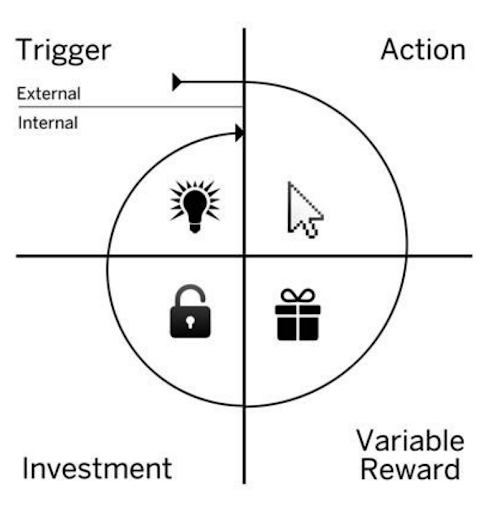
\includegraphics[width = .6\textwidth]{images/hook.png}
    \caption{4 Phasen des Hakenmodells: Auslöser, Aktion, variable Belohnung und Investition} \cite[S. 9]{Eyal2014}
    \label{fig:hooks}
\end{figure}

\noindent Dieses Modell erweist sich für viele unterschiedliche Fallbeispiele als treffende Abbildung des menschlichen Verhaltens im Umgang mit sehr erfolgreichen digitalen Produkten, und könnte für Lightbulb Learning im Folgenden noch bewusster und unmittelbarer angewendet werden. Konkret bedeutet das beispielsweise, dass die äußeren Auslöser, die aktuell vollständig fehlen, in Form von automatisierten E-Mails umgesetzt werden könnten. Auch die variable Belohnung für die Interaktion mit dem System fehlt zum aktuellen Zeitpunkt noch. Hier könnte etwa mit animierten Fortschrittsbalken und Badges bei der Erreichung bestimmter Ziele Abhilfe geschaffen werden. Auch das Liken von Fragen und Antworten könnte mit einer schönen, grafischen Animation belohnt werden.

\subsection{Legal-Themen}
Ein bisher vollständig ausgeblendeter Bereich des Produkt Lightbulb Learning ist die Erfüllung rechtlicher Anforderungen wie einer Datenschutzerklärung und den Nutzungsbedingungen. Für dieses Aufgabe ist zum Zeitpunkt der Abgabe noch kein technologisches Werkzeug, etwa ein open source legal text generator oder ähnliches bekannt, so dass hier noch eine Strategie erdacht und umgesetzt werden muss.

\subsection{Lightbulb Learning Zertifikate}
Das Ziel für Lightbulb Learning, über diese Thesis hinaus, ist die wirtschaftliche Verselbstständigung des Projekts. Die dafür benötigten Einnahmen sollen aus den Zertifikaten entstehen, wie es im Kapitel \ref{sub:certs} bereits beschrieben wurde. Dieses Geschäftsmodell muss noch weiter validiert werden, indem mehr Feedback von Anbietern von Online-Kursen eingeholt wird, und auf dieser Grundlage das Feature mit Einbeziehung eines Bezahl-Dienstleisters umgesetzt wird. Ob Nutzer dafür bereit sind, sich auf Lightbulb Learning einzulassen, hängt im wesentlichen von zwei Faktoren ab: Glauben sie, dass sie mit Lightbulb Learning effektiv lernen können und glauben sie, dass das daraus resultierende Resultat von Wert ist. Mangelt es an der pädagogischen Überzeugtheit, so werden nur wenige Menschen überhaupt mit der Plattform interagieren. Fehlt es an subjektiver Wertschätzung der auszugebenden Zertifikate, so werden nach Erreichung der Qualifikation für das Zertifikat nur wenige Menschen dieses käuflich erwerben. Somit sind die Sicherstellung dieser zwei Aspekte die großen Herausforderungen für Lightbulb Learning nach der Thesis.